\documentclass[11pt]{article}
\usepackage[margin=1in]{geometry}
\usepackage{booktabs}
\usepackage{longtable}
\usepackage{array}
\usepackage{graphicx}
\usepackage{float}
\usepackage{setspace}
\usepackage[hidelinks]{hyperref}
\setlength{\parindent}{0pt}
\begin{document}
\title{Mixed-Effects Analysis of Adjusted Cybercrime Rates}
\author{Automated analysis script}
\date{\today}
\maketitle
\section{Source data and reshaping}
The source workbook was \texttt{ComputerCrime\_AUG2026\_Impact\_Final\_With\_C5C7\_IFERROR\_CHARTS\_FIXED\_UPDATED.xlsx}. The script extracted the seven annual observations (2016--2022) from the Chattanooga-adjusted summary sheets for American Samoa, Tennessee, and California, then reshaped the eleven cybercrime categories into long format.
The long-format dataset contains 231 state-year-category rows. 1 workbook error cell was read as missing, so 230 complete observations were used in the mixed-effects model.
The excluded row was State CA, Year 2016, Category Threats/Stalking/Harassment/Terrorism.
\section{Model specification}
The fitted model used State and Category as fixed effects, included their interaction so that within-category contrasts could be estimated directly, and modeled Year as a random intercept:
\[
\mathrm{AdjustedRate}_{ijk} = \beta_0 + \beta_{\mathrm{State}_i} + \beta_{\mathrm{Category}_j} + \beta_{\mathrm{State}\times\mathrm{Category}_{ij}} + b_{\mathrm{Year}_k} + \varepsilon_{ijk}
\]
\section{Type III tests of fixed effects}
\begin{longtable}{lrrrrrr}
\caption{Type III tests of fixed effects from the mixed-effects model.}\label{tab:type3}\\
\toprule
Effect & Sum Sq & Mean Sq & NumDF & DenDF & F value & Pr(>F) \\
\midrule
\endfirsthead
\toprule
Effect & Sum Sq & Mean Sq & NumDF & DenDF & F value & Pr(>F) \\
\midrule
\endhead
State & 1,516.887 & 758.443 & 2 & 191.02 & 32.688 & <0.001 \\
Category & 6,371.227 & 637.123 & 10 & 191.02 & 27.459 & <0.001 \\
State:Category & 2,125.049 & 106.252 & 20 & 191.02 & 4.579 & <0.001 \\
\bottomrule
\end{longtable}
\section{Estimated marginal means}
\begin{longtable}{p{0.33\linewidth}lrrrrr}
\caption{Estimated marginal means by state within category.}\label{tab:emmeans}\\
\toprule
Category & State & emmean & SE & df & lower.CL & upper.CL \\
\midrule
\endfirsthead
\toprule
Category & State & emmean & SE & df & lower.CL & upper.CL \\
\midrule
\endhead
Data Breach & AS & 0.429 & 1.889 & 169.87 & -3.300 & 4.157 \\
Data Breach & TN & 0.429 & 1.889 & 169.87 & -3.300 & 4.157 \\
Data Breach & CA & 1.000 & 1.889 & 169.87 & -2.728 & 4.728 \\
Personal Data Breach & AS & 5.286 & 1.889 & 169.87 & 1.557 & 9.014 \\
Personal Data Breach & TN & 14.714 & 1.889 & 169.87 & 10.986 & 18.443 \\
Personal Data Breach & CA & 25.714 & 1.889 & 169.87 & 21.986 & 29.443 \\
Malware & AS & 0.857 & 1.889 & 169.87 & -2.871 & 4.586 \\
Malware & TN & 0.429 & 1.889 & 169.87 & -3.300 & 4.157 \\
Malware & CA & 0.571 & 1.889 & 169.87 & -3.157 & 4.300 \\
Phishing & AS & 2.571 & 1.889 & 169.87 & -1.157 & 6.300 \\
Phishing & TN & 8.429 & 1.889 & 169.87 & 4.700 & 12.157 \\
Phishing & CA & 12.000 & 1.889 & 169.87 & 8.272 & 15.728 \\
Ransomware & AS & 0.000 & 1.889 & 169.87 & -3.728 & 3.728 \\
Ransomware & TN & 0.286 & 1.889 & 169.87 & -3.443 & 4.014 \\
Ransomware & CA & 1.000 & 1.889 & 169.87 & -2.728 & 4.728 \\
Crimes Against Children & AS & 1.571 & 1.889 & 169.87 & -2.157 & 5.300 \\
Crimes Against Children & TN & 0.286 & 1.889 & 169.87 & -3.443 & 4.014 \\
Crimes Against Children & CA & 0.429 & 1.889 & 169.87 & -3.300 & 4.157 \\
Extortion & AS & 4.714 & 1.889 & 169.87 & 0.986 & 8.443 \\
Extortion & TN & 14.857 & 1.889 & 169.87 & 11.129 & 18.586 \\
Extortion & CA & 22.571 & 1.889 & 169.87 & 18.843 & 26.300 \\
Threats/Stalking/Harassment/Terrorism & AS & 7.286 & 1.889 & 169.87 & 3.557 & 11.014 \\
Threats/Stalking/Harassment/Terrorism & TN & 5.000 & 1.889 & 169.87 & 1.272 & 8.728 \\
Threats/Stalking/Harassment/Terrorism & CA & 9.000 & 2.034 & 177.88 & 4.987 & 13.013 \\
IPR/Counterfeit & AS & 0.429 & 1.889 & 169.87 & -3.300 & 4.157 \\
IPR/Counterfeit & TN & 0.714 & 1.889 & 169.87 & -3.014 & 4.443 \\
IPR/Counterfeit & CA & 1.286 & 1.889 & 169.87 & -2.443 & 5.014 \\
Identity Theft & AS & 1.857 & 1.889 & 169.87 & -1.871 & 5.586 \\
Identity Theft & TN & 9.857 & 1.889 & 169.87 & 6.129 & 13.586 \\
Identity Theft & CA & 11.857 & 1.889 & 169.87 & 8.129 & 15.586 \\
BEC & AS & 4.000 & 1.889 & 169.87 & 0.272 & 7.728 \\
BEC & TN & 6.714 & 1.889 & 169.87 & 2.986 & 10.443 \\
BEC & CA & 12.857 & 1.889 & 169.87 & 9.129 & 16.586 \\
\bottomrule
\end{longtable}
\section{Planned contrasts}
The planned contrasts were Tennessee versus American Samoa and Tennessee versus California within each category, with no multiplicity adjustment because the comparisons were prespecified.
\begin{longtable}{p{0.30\linewidth}lrrrrrr}
\caption{Planned contrasts comparing Tennessee with American Samoa and California within each category.}\label{tab:contrasts}\\
\toprule
Category & contrast & estimate & SE & df & lower.CL & upper.CL & p.value \\
\midrule
\endfirsthead
\toprule
Category & contrast & estimate & SE & df & lower.CL & upper.CL & p.value \\
\midrule
\endhead
Data Breach & TN vs AS & -0.000 & 2.575 & 191.00 & -5.079 & 5.079 & 1.000 \\
Data Breach & TN vs CA & -0.571 & 2.575 & 191.00 & -5.650 & 4.507 & 0.825 \\
Personal Data Breach & TN vs AS & 9.429 & 2.575 & 191.00 & 4.350 & 14.507 & <0.001 \\
Personal Data Breach & TN vs CA & -11.000 & 2.575 & 191.00 & -16.079 & -5.921 & <0.001 \\
Malware & TN vs AS & -0.429 & 2.575 & 191.00 & -5.507 & 4.650 & 0.868 \\
Malware & TN vs CA & -0.143 & 2.575 & 191.00 & -5.221 & 4.936 & 0.956 \\
Phishing & TN vs AS & 5.857 & 2.575 & 191.00 & 0.779 & 10.936 & 0.024 \\
Phishing & TN vs CA & -3.571 & 2.575 & 191.00 & -8.650 & 1.507 & 0.167 \\
Ransomware & TN vs AS & 0.286 & 2.575 & 191.00 & -4.793 & 5.364 & 0.912 \\
Ransomware & TN vs CA & -0.714 & 2.575 & 191.00 & -5.793 & 4.364 & 0.782 \\
Crimes Against Children & TN vs AS & -1.286 & 2.575 & 191.00 & -6.364 & 3.793 & 0.618 \\
Crimes Against Children & TN vs CA & -0.143 & 2.575 & 191.00 & -5.221 & 4.936 & 0.956 \\
Extortion & TN vs AS & 10.143 & 2.575 & 191.00 & 5.064 & 15.221 & <0.001 \\
Extortion & TN vs CA & -7.714 & 2.575 & 191.00 & -12.793 & -2.636 & 0.003 \\
Threats/Stalking/Harassment/Terrorism & TN vs AS & -2.286 & 2.575 & 191.00 & -7.364 & 2.793 & 0.376 \\
Threats/Stalking/Harassment/Terrorism & TN vs CA & -4.000 & 2.683 & 191.26 & -9.292 & 1.291 & 0.138 \\
IPR/Counterfeit & TN vs AS & 0.286 & 2.575 & 191.00 & -4.793 & 5.364 & 0.912 \\
IPR/Counterfeit & TN vs CA & -0.571 & 2.575 & 191.00 & -5.650 & 4.507 & 0.825 \\
Identity Theft & TN vs AS & 8.000 & 2.575 & 191.00 & 2.921 & 13.079 & 0.002 \\
Identity Theft & TN vs CA & -2.000 & 2.575 & 191.00 & -7.079 & 3.079 & 0.438 \\
BEC & TN vs AS & 2.714 & 2.575 & 191.00 & -2.364 & 7.793 & 0.293 \\
BEC & TN vs CA & -6.143 & 2.575 & 191.00 & -11.221 & -1.064 & 0.018 \\
\bottomrule
\end{longtable}
\section{Confidence-interval plots}
\begin{figure}[H]
\centering
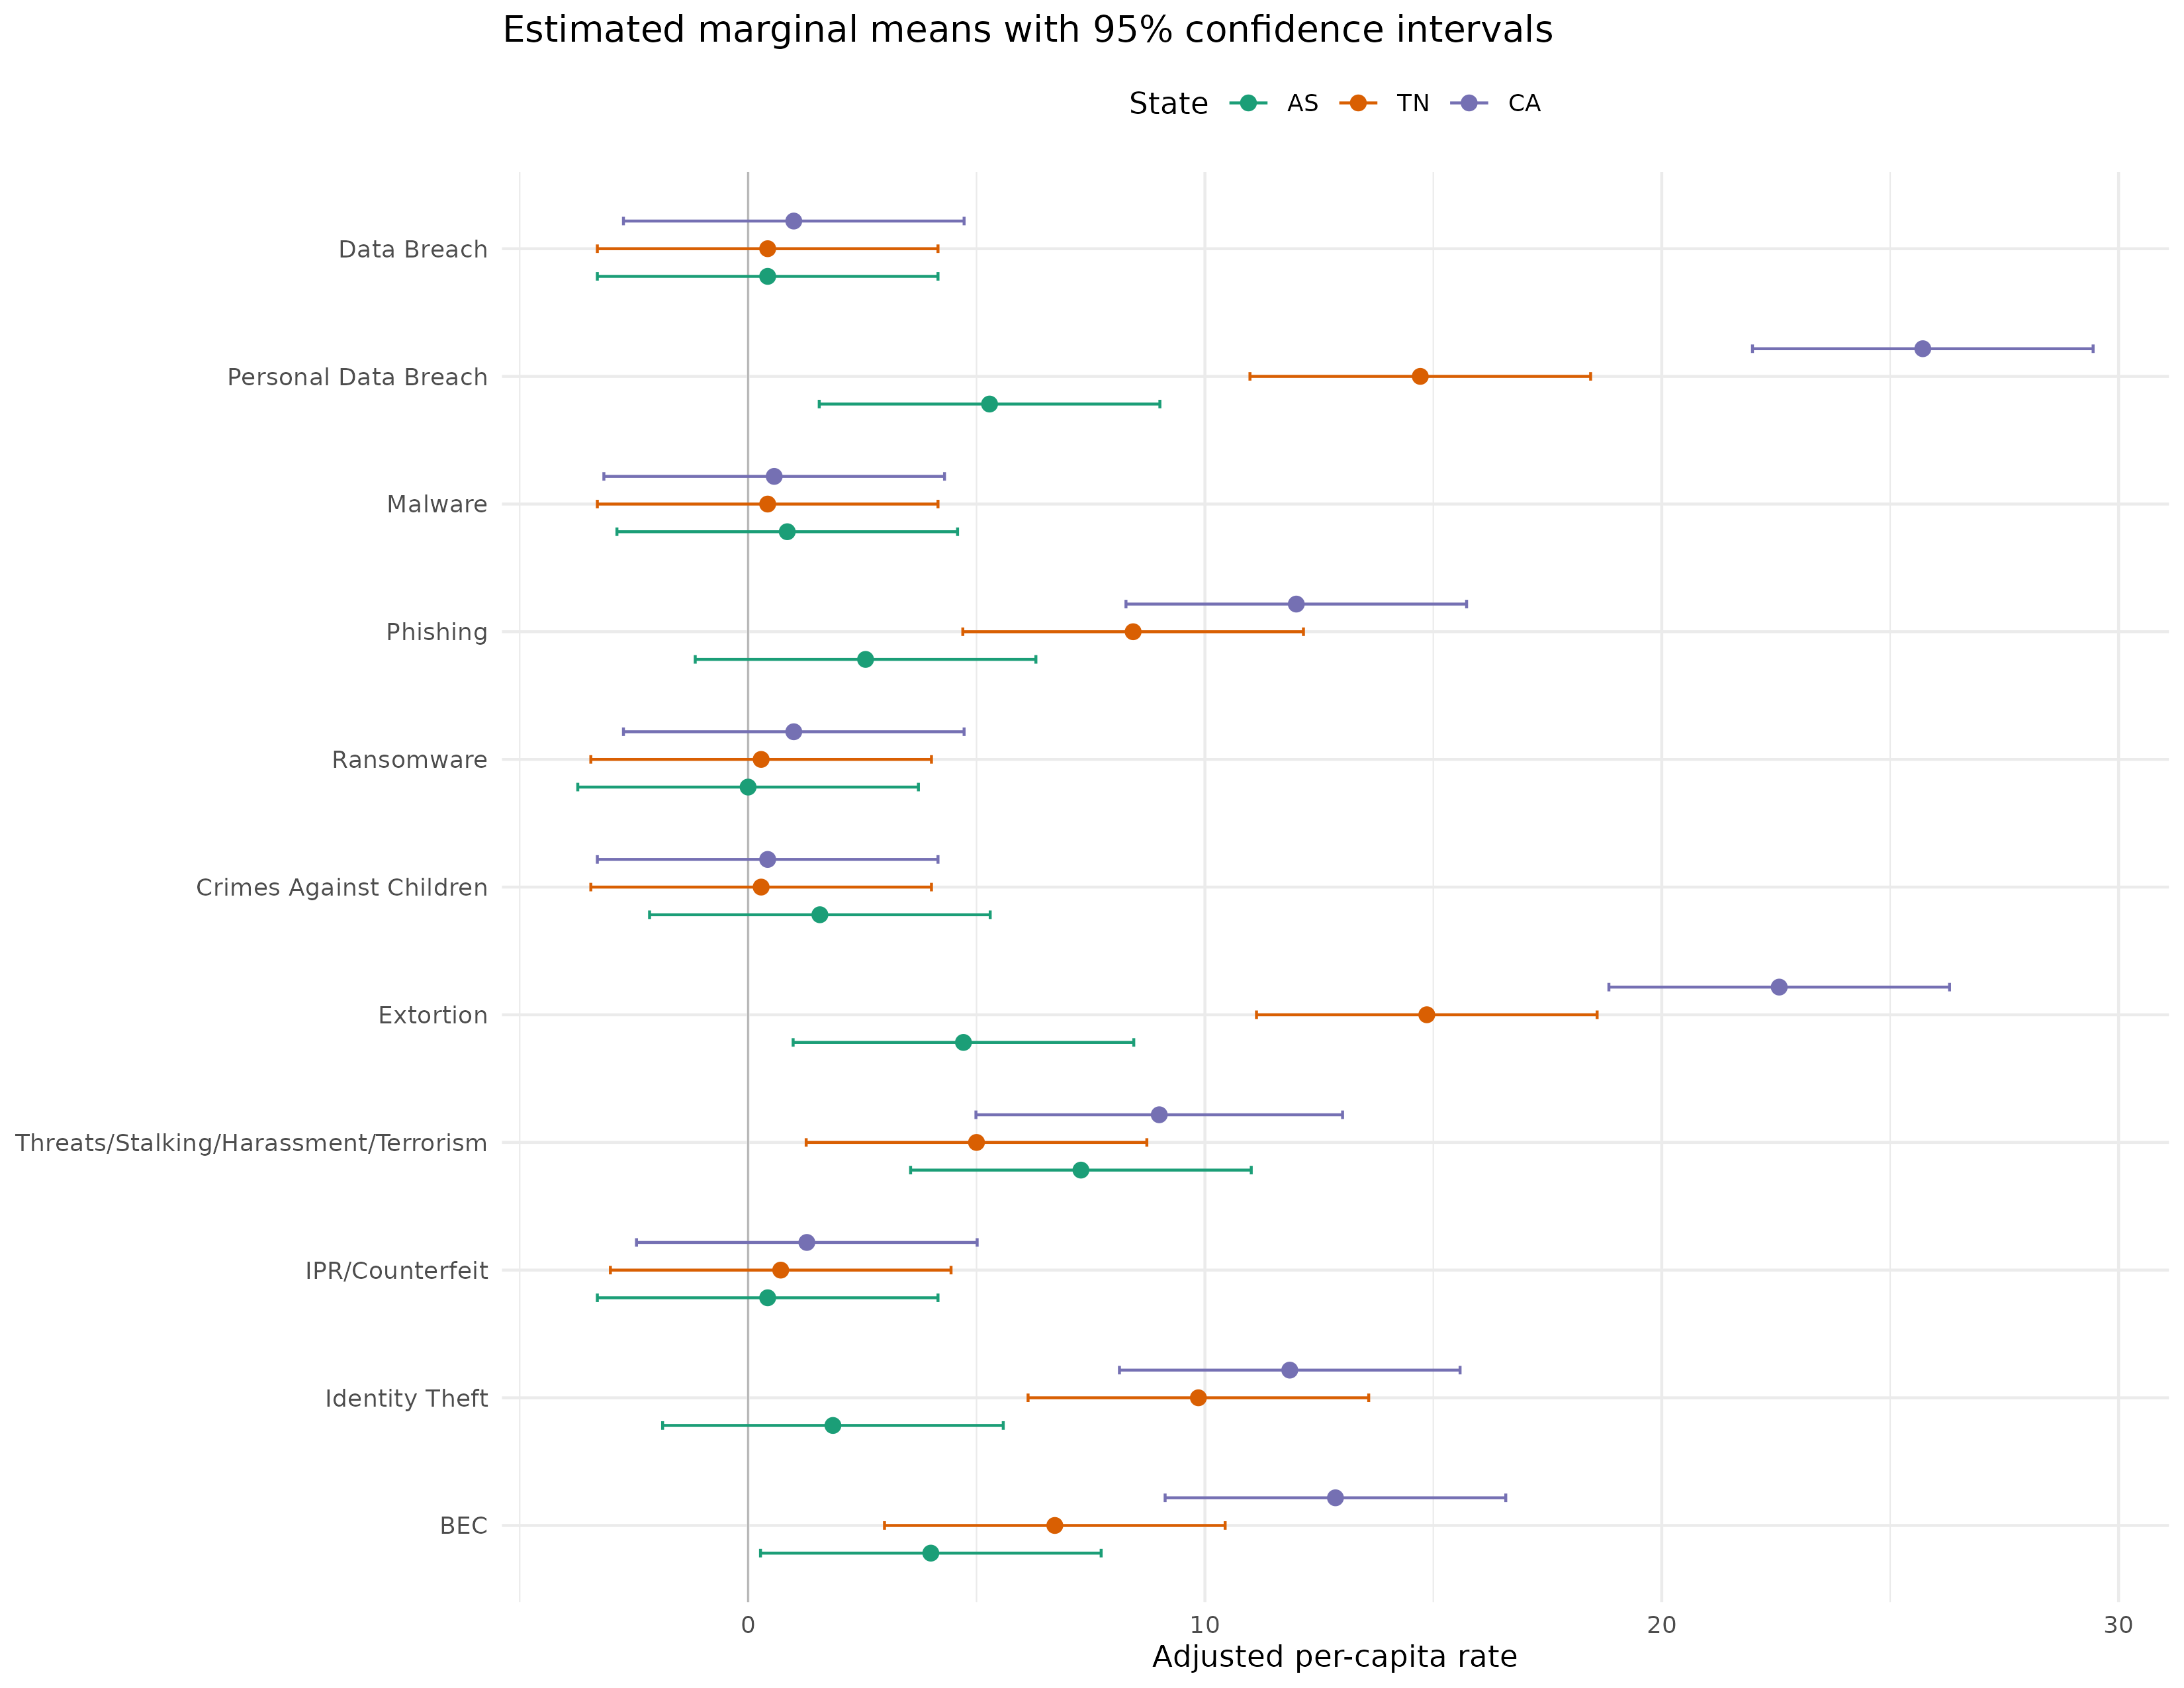
\includegraphics[width=\textwidth]{cybercrime_emmeans_ci.png}
\caption{Estimated marginal means and 95\% confidence intervals.}
\end{figure}
\begin{figure}[H]
\centering
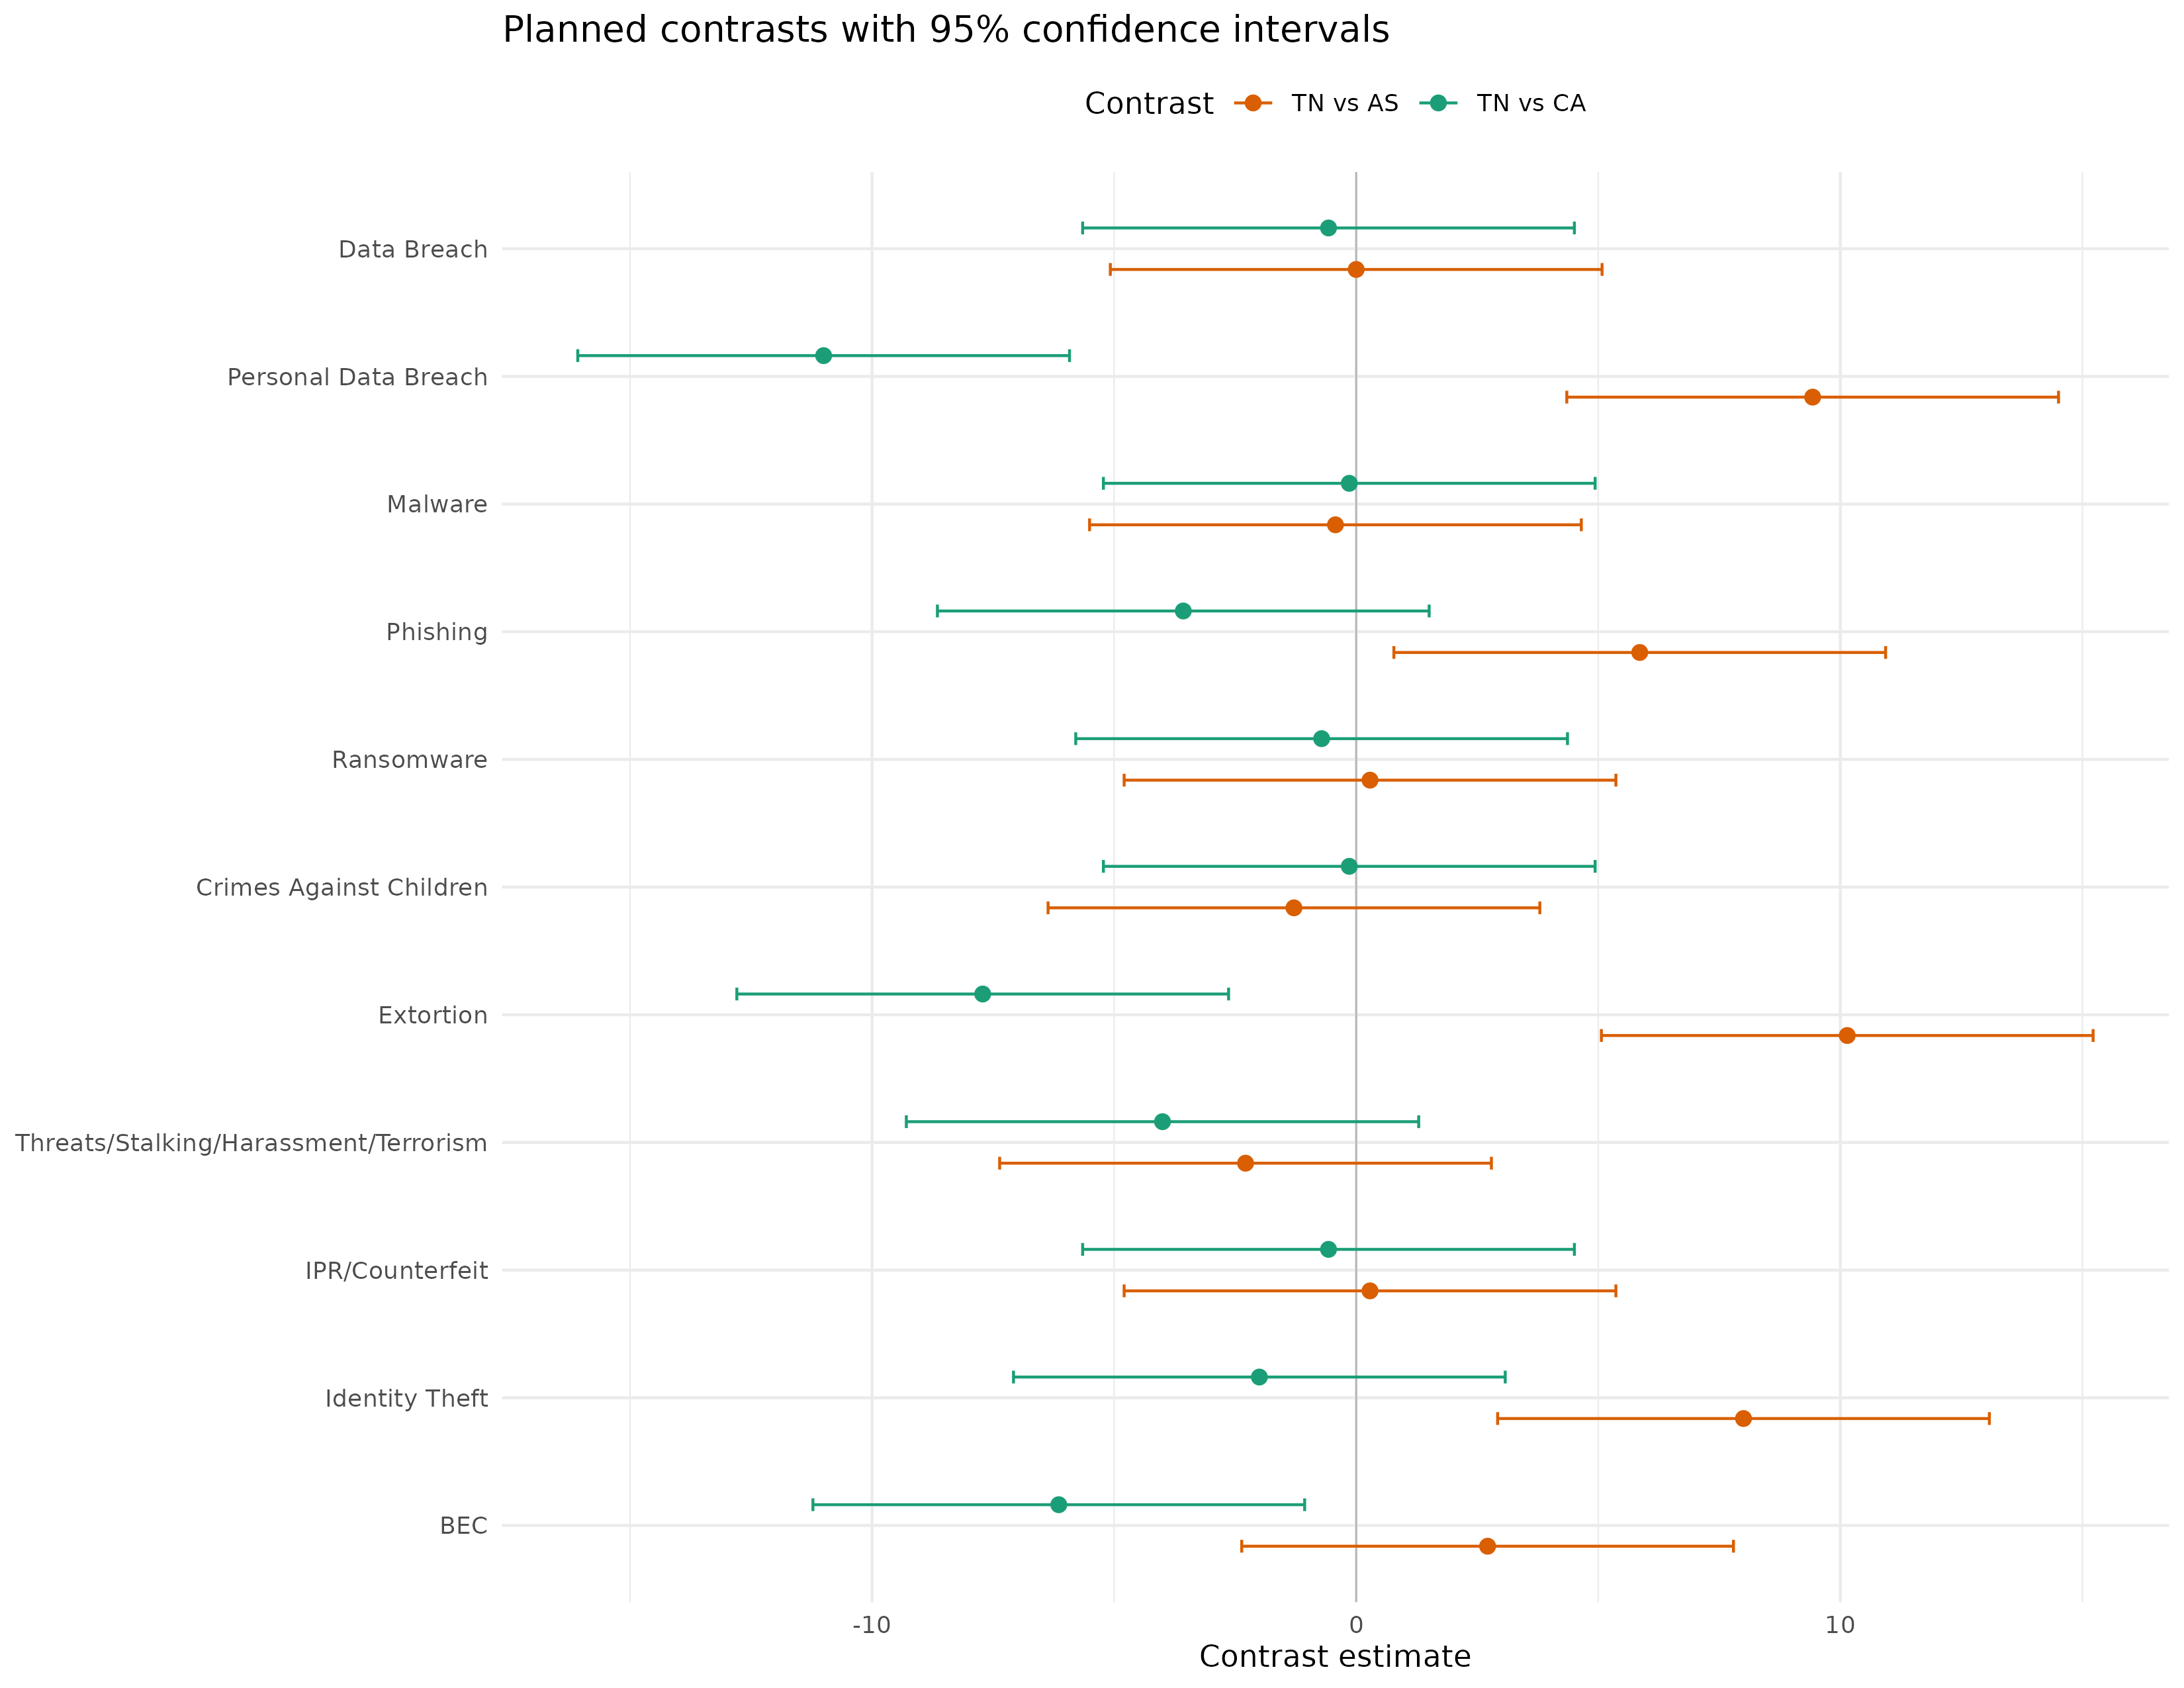
\includegraphics[width=\textwidth]{cybercrime_contrasts_ci.png}
\caption{Planned contrast estimates and 95\% confidence intervals.}
\end{figure}
\end{document}
